\section{Tic-Tac-Toe}

In diesem Abschnitt wird das Strategiespiel Tic-Tac-Toe (\ac{TTT}) erklärt. Anschließend wird begründet, wieso die vorgestellten Algorithmen darauf angewandt werden können. 

\subsection{Spielerklärung}
\acl{TTT} ist ein Strategiespiel, das von zwei Spielern gespielt wird \cite[S. 6]{allisSearchingSolutionsGames1994}.
Das Spielfeld ist unterteilt in neun Bereiche (Slots), die in einer 3x3 Matrix angeordnet sind. 
%Die Slots gehören daher zu einer von drei Klassen, die als Ecken, Kanten oder Mitte bezeichnet werden. Zu Beginn sind alle Slots leer. 
Die Spieler platzieren abwechselnd ihr zugeteiltes Symbol, entweder X oder O, in einem Slot auf dem Spielfeld. 
Der beginnende Spieler verwendet in der Regel das Symbol X. 
Ziel jedes Spielers ist es, drei eigene Symbol entweder vertikal, horizontal oder diagonal in einer Reihe zu platzieren.
Somit gibt es insgesamt acht mögliche Gewinnkonstellationen: drei Zeilen, drei Spalten und zwei Diagonalen. 
Sind alle Slots belegt ohne, dass einer der Spieler gewonnen hat, endet das Spiel in einem Unentschieden. \cite[S. 533]{crowleyFlexibleStrategyUse1993}

\acs{TTT} besitzt 5478 legale Spielfeldkonstellationen und hat im Vergleich zu Spielen wie Schach oder Vier Gewinnt eine deutlich geringere Zustandsraum-Komplexität  \cite[S. 159]{allisSearchingSolutionsGames1994}.
Dies kann sogar weiter reduziert werden, da aufgrund von Rotations- und Spiegelsymmetrien bis zu acht Spielfeldkonstellationen äquivalent sein können.\footnote{4 Rotationen und 4 Spiegelungen, jeweils horizontal/vertikal mit und ohne 90° Drehung} 
Dadurch reduziert sich die Zustandsraum-Komplexität auf 765. \cite[S. 3]{block-berlitzm.ProInformatikFunktionaleProgrammierung2009}

In der Spieltheorie ist \acs{TTT} ein klassisches Beispiel für ein Nullsummenspiel, da ein Gewinn immer mit einer Niederlage für den Gegner einhergeht \cite[S. 6]{allisSearchingSolutionsGames1994}, \cite[S. 533]{crowleyFlexibleStrategyUse1993}.
Zudem gehört TTT zu den Spielen mit perfekter Information, weil beide Spieler Zugriff auf alle Informationen des aktuellen Spielzustands haben \cite[S. 156]{allisSearchingSolutionsGames1994}, \cite[S. 38]{gardnerm.HexaflexagonsOtherMathematical1988}.
\acs{TTT} ist ein stark gelöstes Spiel, \dahe es gibt eine optimale Strategie für jede legale Position \cite[S. 6]{allisSearchingSolutionsGames1994}
Spielen beide Spieler optimal endet TTT immer in einem Unentschieden und wird daher als futile Game (\dt vergebliches Spiel) bezeichnet \cite[S. 177]{wangPopularLecturesMathematical2014}.
Somit ist das beste Spielergebnis immer zu Gewinnen und gegen einen optimalen Spieler Unentschieden zu spielen. 
Regeln für ein perfektes Spiel wurden erstmals 1972 in \cite{newellHumanProblemSolving1972} formuliert. 
\citeauthor{crowleyFlexibleStrategyUse1993} erweiterten diese unter der Bezeichnung \gqq{Model of Expert Performance}, wie im Anhang \cref{chap:ModelofExpert} gelistet \cite[S. 536]{crowleyFlexibleStrategyUse1993}. 
Die folgenden vier Regeln \bzw Aktionen bilden in der dargestellten Reihenfolge die zentrale Strategie für Expert Play. Beispielhafte Spielfeldkonstellationen werden in Abbildung \cref{fig:ttt_expertplay} gezeigt.

\begin{enumerate}
    \item \textbf{Win}: Wenn der Spieler eine Möglichkeit hat zu gewinnen, soll diese genutzt werden
    \item \textbf{Block}: Wenn der Gegner zwei Symbole in einer Reihe hat, blockiere den Gewinn des Gegners
    \item \textbf{Fork}: Wenn sich zwei Reihen schneiden, in denen der Spieler sein Symbol platziert hat und der Slot, wo sie sich schneiden leer ist, belege diesen Slot
    \item \textbf{Block Fork}: Wenn die Möglichkeit besteht, zwei Symbole in eine Reihe zu legen, wähle diesen Slot, um den Gegner zum Blocken zu zwingen. Andernfalls wähle einen Slot, um ein Fork des Gegners zu verhindern
\end{enumerate}

\begin{figure}
    \centering
    \begin{subfigure}[b]{0.45\textwidth}
      \centering
      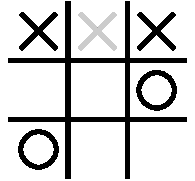
\includegraphics[scale=0.7]{ttt_boards/ttt_win.pdf}
      \caption{Win}
      \label{fig:ttt_win}
    \end{subfigure}
    \begin{subfigure}[b]{0.45\textwidth}
      \centering
      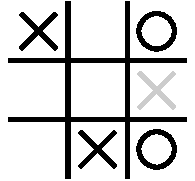
\includegraphics[scale=0.7]{ttt_boards/ttt_block.pdf}
      \caption{Block}
      \label{fig:ttt_block}
    \end{subfigure}
    \begin{subfigure}[b]{0.45\textwidth}
      \centering
      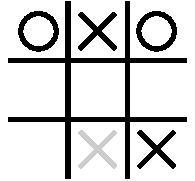
\includegraphics[scale=0.7]{ttt_boards/ttt_fork.pdf}
      \caption{Fork}
      \label{fig:ttt_fork}
    \end{subfigure}
    \begin{subfigure}[b]{0.45\textwidth}
      \centering
      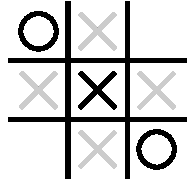
\includegraphics[scale=0.7]{ttt_boards/ttt_blockfork.pdf}
      \caption{Block Fork}
      \label{fig:ttt_blockfork}
    \end{subfigure}
    \caption[Beispielhafte Spielfeldkonstellationen für TTT Expert Play]{Beispielhafte Spielfeldkonstellationen für \acs{TTT} Expert Play. Optimale Aktionen sind grau gefärbt \protect\footnotemark}
    \label{fig:ttt_expertplay}
\end{figure}

\footnotetext{Spielfeldkonstellationen übernommen aus \cite[S. 539]{crowleyFlexibleStrategyUse1993}, Alle \acs{TTT} Spielfelder werden erstellt mit Code von \cite{sebglavCreatingTicTacToeBoards2022}}

Der zweite Teil der Strategie beschäftigt sich mit dem optimalen ersten Zug für X. 
Aufgrund der Äquivalenz der möglichen Aktionen reduziert sich die Auswahl auf drei Möglichkeiten: Ecke, Kante und Mitte. 
In \cite[S. 38]{gardnerm.HexaflexagonsOtherMathematical1988} wird die Ecke als stärkste Aktion dargestellt, da der Gegner mit der Mitte kontern muss, um nicht zu verlieren. 
Hingegen zeigen Studien wie \cite{kutscheraa.BestOpeningMove2018}, dass die Mitte die beste Aktion ist, da diese in der Menge aller möglichen Spielabfolgen die Startposition mit den meisten gewonnen Spielen ist.
Spielen zwei optimale Spieler gegeneinander ist die Wahl der ersten Aktion unbedeutend \cite[S. 38]{gardnerm.HexaflexagonsOtherMathematical1988}.

\subsection{Anwendbare Algorithmen}
\label{sec:anwendbare_algorithmen}
Eine Voraussetzung für die Anwendung des Minimax-Algorithmus ist, dass der Spielbaum eine geringe Komplexität hat \cite[S. 10]{block-berlitzm.ProInformatikFunktionaleProgrammierung2009}.
Die Spielbaum-Komplexität ist definiert als die Anzahl der Terminalknoten des vollständig konstruierten Spielbaums und wird angegeben als $\log$ zur Basis $10$ \cite[S. 160]{allisSearchingSolutionsGames1994}.
Aufgrund des kleinen Zustands- und Aktionsraums von \ac{TTT}, ist dessen Spielbaum klein.
Die Spielbaum-Komplexität beträgt $5$ ist im Vergleich zu Spielen wie Schach (123) oder Shogi (226) relativ gering \cite[S. 11]{block-berlitzm.ProInformatikFunktionaleProgrammierung2009}.
Somit erfüllt \ac{TTT} diese Bedingung für die Anwendung des Minimax-Algorithmus.
Eine weitere Bedingung des Minimax-Algorithmus ist, dass das Spiel ein Zweispieler-Nullsummenspiel mit perfekter Information sein muss \cite[S. 10]{block-berlitzm.ProInformatikFunktionaleProgrammierung2009}. 
Da \ac{TTT} auch diese Bedingung erfüllt, kann der Minimax-Algorithmus angewendet werden.
In \cref{fig:ttt_tree} ist ein Auszug des Spielbaums von \acs{TTT} mit der möglichen Umsetzung eines Minimax-Algorithmus dargestellt. Jedoch ist anzumerken, dass der Minimax-Algorithmus einen optimalen Gegner erwartet und daher nur gegen diese optimal spielt. Minimax kann nicht verlieren, aber wählt seine Aktionen nicht, um seine Gewinnwahrscheinlichkeit gegen nicht optimale Spieler zu maximieren. \cite[S. 8]{suttonLearningPredictMethods1988}. 

Voraussetzung für die Anwendung von \ac{TDL} Algorithmen ist, dass das zu lösende Problem als \ac{MDP} formuliert werden kann.
Der mögliche Zustandsraum $S$ und Aktionsraum $A$ sind für \ac{TTT} diskret und bekannt. 
Da \ac{TTT} ein Spiel mit perfekter Information ist, kann bei gegebenem Zustand $s$ und Aktion $a$ der Folgezustand $s'$ bestimmt werden.
Somit erfüllt \ac{TTT} die Markov Eigenschaft und kann als ein \ac{MDP} modelliert werden.
Die weitere Voraussetzung ist, dass der Agent mit seiner Umgebung interagieren kann und von dieser Samples in Form des Tupels $(S_t,A_t,R_{t+1},S_{t+1})$ erhält. \cite[S. 88]{kontesg.SeminarReinforcementLearning2021}
Diese kann im Rahmen der Implementierung beachtet werden. 
Da somit beide Voraussetzungen erfüllt sind, können \ac{TDL} Methoden wie \bothAlgs angewendet werden.

\begin{figure}[h]
    \centering
    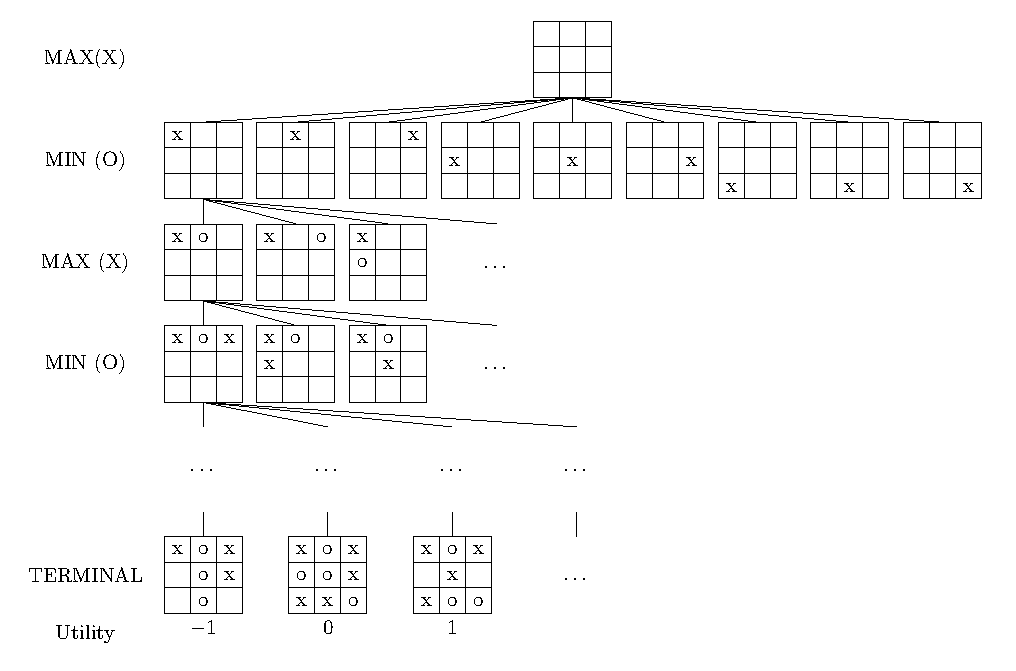
\includegraphics[scale=0.7]{04_Artefakte/01_Abbildungen/ttt_boards/ttt_tree.pdf}
    \caption[Auszug aus dem Spielbaum von \acs{TTT}]{Auszug aus dem Spielbaum von \acs{TTT} \protect\footnotemark}
    \label{fig:ttt_tree}
\end{figure}

\footnotetext{Darstellung übernommen aus \cite[S. 125]{russellArtificialIntelligenceModern2021}, Abbildung erstellt mit Code von \cite{vj.l.TikzPgfFollowup}}